\ItemCategory{}
\ItemSubCategory{}
\ItemFolder{}

\chapter*{Amulet of Justice}\stepcounter{section}\phantomsection\addcontentsline{toc}{section}{Amulet of Justice}
\itemDescriptionAndImage{Wondrous Item, legendary (requires attunement)}{images/Magic_Items/Amulet_of_Justice.png}{9.5cm}\\

\begin{tikzpicture}[remember picture, overlay]%
	\node[xshift=0.5\columnwidth, yshift=-0.35\paperheight] at (current page.center) {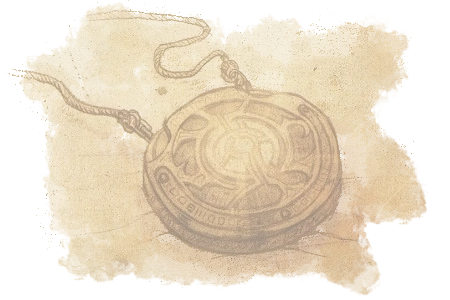
\includegraphics[width=1.75\columnwidth]{%
		images/Magic_Items/Amulet_of_Justice_background.png%
	}};%
\end{tikzpicture}%
	
\section*{Appearance}
{\entryfont The Amulet of Justice is a breathtaking artifact, its body crafted entirely from pure, lustrous silk that gleams with a subtle, otherworldly radiance. The silk is tightly woven and shaped into a smooth, flowing form that seems impossibly durable despite its delicate appearance. At the heart of the amulet rests a striking gem, as white and pristine as freshly fallen snow, radiating a soft, calming glow. The silk's edges are adorned with faint, shimmering patterns that resemble ancient runes or flowing streams, giving the amulet an aura of mystique and purpose. The white gem, seamlessly embedded in the silk, draws the eye and exudes an air of quiet, undeniable power, as if it holds the very essence of justice within its core.}

\section*{History}
{\entryfont The origins of the Amulet of Justice are steeped in mystery, its creation lost to time and whispers of forgotten lore. Tales speak of a powerful artifact forged by divine hands or ancient, unrecorded magic, though none can say for certain. What is known is that its location is a well-guarded secret, known only to an enigmatic magic-wielding blue dragon named Thaloryx, Seeker of Justice, who dwells in the craggy heights of Strathclyde. Thaloryx safeguards the knowledge of the amulet's resting place - hidden deep beneath the tranquil waters of Loch Rannoch, a place said to be warded by enchantments that deter even the boldest of seekers.}

\section*{Magic}
{\entryfont The Amulet of Justice is a powerful artifact imbued with ancient, restorative magic that serves as a counterbalance to dark forces. Its primary ability is to directly oppose and neutralize the malevolent enchantments of the infamous "Knife of Evil." When activated, the amulet emits a radiant light that pierces through shadows of corruption, unraveling the sinister spells cast by the blade. This power allows it to reverse curses, dispel harmful effects, and mend the damage wrought by the knife's influence. The amulet's magic is precise, targeting the specific threads of evil magic and restoring balance and purity to those afflicted. It is said that the gem at its center glows brighter when its restorative magic is in use, embodying the unwavering light of justice triumphing over darkness.}

\subsection*{Gameplay Mechanics}
{\entryfont While attuned to the Amulet of Justice, the wearer is shielded from the curse of the Knife of Evil, and any curses already affecting the wearer are ended and has advantage on saving throws against being frightened or charmed. Additionally, while attuned, the wearer can use an action to touch a willing creature. The touched creature must succeed on a DC 20 Wisdom saving throw (DC 15 if the wearer has reached level 10). On a success, any curse affecting the creature is suppressed until the end of their next turn. This suppression also applies to the Charmed and Frightened conditions.

If the creature succeeds on the saving throw, they can repeat the Wisdom saving throw at the end of each of their turns to extend the effect for one additional turn. Only one creature can benefit from this effect at a time (this limit increases to two creatures at 5th level, three creatures at 11th level, and four creatures at 17th level).}